\pagebreak
\section{Cursograma de Cobranzas}
La empresa posee distintas formas de cobros, las cuales varian con el cliente. Algunas clientes pagan a traves de una cuenta corriente con una transferencia, otros con cheque o efectivo. A determinados clientes se les envía un cobrador mientras que muchos otros no.
Por simplicidad, en este caso se describe el caso en el cual el cliente se acerca a la empresa al sector de finanzas a entregar los valores (cheques o efectivo).

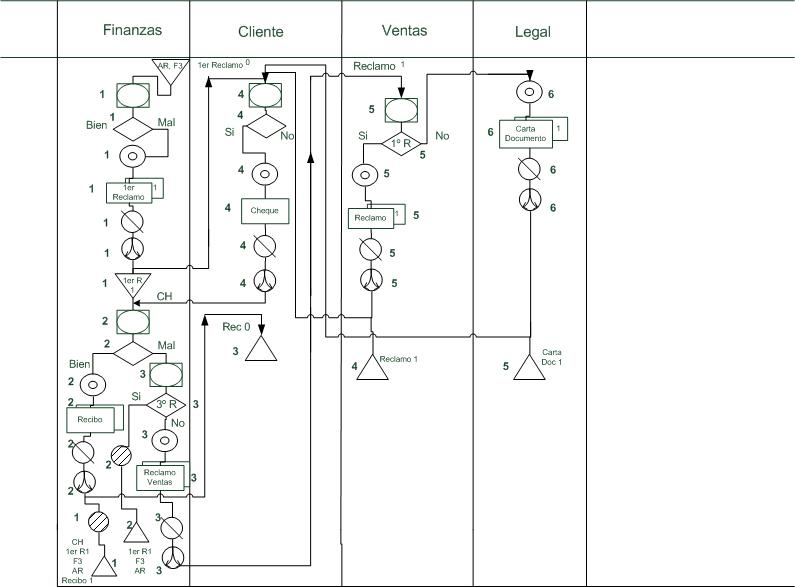
\includegraphics[scale=0.8]{Empresa/Circuitos/Cobranzas/cursograma-para-manual-cobranzas-3.jpg}

\pagebreak
\section{Procedimiento de Cobranzas}
\begin{enumerate}
  \item \textbf{Finanzas:} ejecuta un reporte en el sistema, el cual trae todas las facturas que vencen a la fecha. De ellas selecciona aquellas que no han sido pagadas. Esta tarea se realiza todos los días.
  Por cada factura vencida que no este paga, emite un reclamo del pago por duplicado, con una fecha de vencimiento de pago. El primero lo firma y se lo envía al cliente. El otro lo archiva para que quede constancia del reclamo.
  \item \textbf{Cliente:} recibe el reclamo o carta de documento, y en caso de pagar, confecciona un cheque para realizar el mismo y lo envia al sector de finanzas.
  \item \textbf{Finanzas:} en caso de recibir el cheque, revisa que corresponda con la cantidad a pagar y que este correctamente confeccionado. Si este esta correcto, emite un recibo por duplicado, firma el original y se lo entrega al cliente. Finalmente, archiva el cheque, la factura por triplicado, el duplicado del reclamo y registra en el sistema el pago de la factura.
  Si el cliente no paga, emite un reclamo a ventas y se lo envia a dicho sector. Si ya es la tercera vez que el cliente no paga, archiva los documentos utilizados y asienta en el sistema la falta de pago en la cuenta \textit{pérdidas}.
  \item \textbf{Ventas:} recibe el reclamo y si es la primera vez que se recibe un reclamo emite un segundo reclamo al cliente por duplicado. Firma el original y lo envia al cliente con una fecha límite para el pago. Si no es la primera vez que recibe un reclamo de finanzas, avisa de al sector legal de la falta de pago del cliente de manera informal(mail, llamado telefónico).
  \item \textbf{Legal:} una vez notificado de la falta de pago del cliente, emite una carta de documento, intimando al cliente a pagar las facturas que debe. La carta de documento es enviada al domicilio legal del cliente de forma tal que quede notificado.
\end{enumerate}

\pagebreak
\section{Manual del Cursograma de Cobranzas}

\begin{center}\textbf{Sectores intervinientes}\end{center}
\begin{itemize}
  \item Finanzas
  \item Ventas
  \item Cliente
  \item Legal
\end{itemize}

\begin{center}
  \textbf{Documentos}
  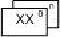
\includegraphics{./Images/Simbolos/simbolo-Documentos.png}
\end{center}
\begin{enumerate}
\item Reclamo a Cliente
\item Reclamo a Ventas
\item Cheque
\item Recibo
\item Carta Documento
\end{enumerate}

\begin{center}
  \textbf{Emisión de Documentos}
  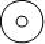
\includegraphics{./Images/Simbolos/simbolo-Emision-de-Documentos.png}
\end{center}
\begin{enumerate}
\item Finanzas: Emite primer Reclamo a Cliente por original y copia.
\item Finanzas: Emite Recibo por original y copia.
\item Finanzas: Emite Reclamo a Ventas.
\item Cliente: Emite Cheque.
\item Ventas: Emite segundo y tercer Reclamo a Cliente por original y copia.
\item Legal: Emite Carta Documento por original y copia.
\end{enumerate}

\begin{center}
  \textbf{Firma}
  
\includegraphics{./Images/Simbolos/simbolo-Firma.png}
\end{center}
\begin{enumerate}
\item Finanzas: Firma el original del primer Reclamo a Cliente.
\item Finanzas: Firma recibo oringinal con la entrega del cheque.
\item Finanzas: Firma el Reclamo a Ventas y se lo envia a dicho sector.
\item Cliente: Firma el cheque que luego entrega contra recibo a Finanzas.
\item Ventas: Firma el original del segundo o tercer Reclamo a Cliente.
\item Legal: Firma original de Carta Documento con la que notifica al cliente de la falta de pago.
\end{enumerate}

\begin{center}
  \textbf{Distribución}
  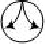
\includegraphics{./Images/Simbolos/simbolo-Distribucion.png}
\end{center}
\begin{enumerate}
\item Finanzas: distribuye el original del primer Reclamo a Cliente al cliente y conserva el duplicado.
\item Finanzas: entrega el recibo original a cambio del cheque recibido y conserva el duplicado del recibo.
\item Finanzas: distribuye el Reclamo a Ventas al sector de Ventas.
\item Cliente: entrega el cheque contra recibo.
\item Ventas: distribuye el original del segundo o tercer Reclamo a Cliente al cliente y conserva el duplicado.
\item Legal: Firma el original de Carta Documento y conserva el duplicado.
\end{enumerate}

\begin{center}
  \textbf{Almacenamiento Transitorio}
  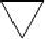
\includegraphics{./Images/Simbolos/simbolo-Almacenamiento-Transitorio.png}
\end{center}
\begin{enumerate}
\item Finanzas: almacena copia del primer Reclamo a Cliente.
\end{enumerate}

\begin{center}
  \textbf{Control y verificación}
  
\includegraphics{./Images/Simbolos/simbolo-Control-y-Verificacion.png}
\end{center}
\begin{enumerate}
\item Finanzas: Ejecuta un reporte en el sistema donde saca las facturas ya vencidas que no estan pagas. Controla el resultado del mismo con las factura por triplicado que tiene archivadas.
\item Finanzas: Verifica que el cheque que le fue entregado por el Cliente este correctamente confeccionado y se corresponda con el monto que indica la factura por triplicado que posee.
\item Finanzas: Luego de un tiempo controla si el Cliente pago o no el reclamo correspondiente. Verifica si el ya es el tercer reclamo que se le hizo al cliente.
\item Cliente: Verifica que sea correcta la factura que se le esta reclamando, y que se corresponda con lo que el mismo posee en sus registros y documentos.
\item Ventas: Ventas verifica si es el primer o segundo reclamo que le ha llegado por parte de una misma factura de ese cliente.
\end{enumerate}

\begin{center}
  \textbf{Decisión}
  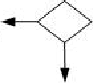
\includegraphics{./Images/Simbolos/simbolo-Decision.png}
\end{center}
\begin{enumerate}
\item Finanzas: Una vez que el resultado del reporte de facturas vencidas y que estas esten correctas emite los correspondientes reclamos para el cliente. Si no, no hace nada ( no hay facturas a cobrar).
\item Finanzas: Si el cheque recibido esta bien hecho y se corresponde con el monto de la factura vencida, procede a emitir el recibo correspondiente. Si el cliente no paga, venciendose el plazo de la factura o reclamo, procede a verificar si ya se han emitido otros reclamos o no.
\item Finanzas: Si ya era el tercer reclamo que se le envio al cliente, procede a asentar la falta de pago en el sistema. Si no, emite el primer o segundo reclamo correspondiente a Ventas.
\item Cliente: Una vez verificada la factura que se le reclama decide en caso de estar correcta la misma, confeccionar el cheque para realizar el pago. En caso contrario no hace nada (o depende de cada cliente, en realidad no interesa que hace si no paga).
\item Ventas: Una vez verificado el reclamo proveniente de Finanzas, y que este este correcto emite un Reclamo a Cliente. Si este no era el primer reclamo que venia del sector de Ventas, notifica de la falta de pago a Legal para que emita la Carta Documento.
\end{enumerate}

\begin{center}
  \textbf{Registro}
  
\includegraphics{./Images/Simbolos/simbolo-Registro.png}
\end{center}
\begin{enumerate}
\item Finanzas: registra en el sistema el cobro en la cuenta \textit{cobros}.
\item Finanzas: registra en el sistema el la falta de pago en la cuenta \textit{pérdidas}.
\end{enumerate}

\begin{center}
  \textbf{Almacenamiento definitivo}
  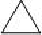
\includegraphics{./Images/Simbolos/simbolo-Almacenamiento-Definitivo.png}
\end{center}
\begin{enumerate}
\item Finanzas: archiva el cheque, el duplicado del recibo, el duplicado del primer Reclamo a Cliente y el triplicado de la factura.
\item Finanzas: archiva el duplicado del primer Reclamo a Cliente y el triplicado de la factura.
\item Cliente: archiva el original del recibo.
\item Ventas: almacena copia del segundo y/o tercer Reclamo a Cliente.
\item Legal: almacena copia de Carta Documento.
\end{enumerate}

\pagebreak
\section{Formularios de Cobranzas}

\subsection{Listado de Cobranzas}
\begin{center}
  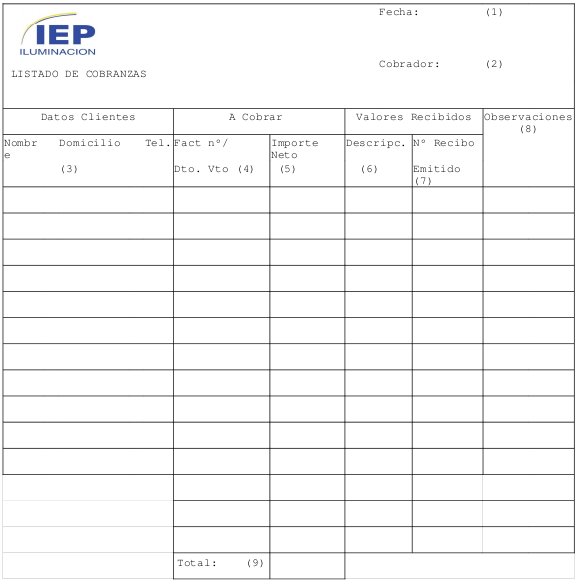
\includegraphics[scale=0.6]{./Images/FormulariosIEP/listado_cobranzas_IEP.png}
\end{center}

\begin{itemize}
  \item \textbf{Objetivo:} Documento que facilita el trabajo del Cobrador. Le indica los cobros que debe realizar, el lugar, el monto y las facturas a cobrar.
  \item \textbf{Alcance:} Este documento lo confecciona finanzas para el cobrador.
  \item \textbf{Emisor:} Finanzas
  \item \textbf{Cantidad de Copias Emitidas:} 0
  \item \textbf{Sector receptor:} Cobrador
 \end{itemize}
 
\subsubsection{Descripci\'on campos del Listado de Cobranzas}
\begin{enumerate}
\item Fecha de Emisión de Listado de Cobranzas
\item Nombre de la persona encargada de cobrar
\item Datos del cliente: Nombre , Domicilio, Teléfono
\item Numero de la factura a cobrar y su respectivo vencimiento
\item Importe neto de la factura a cobrar
\item Descripción de los valores recibidos
\item Numero de recibo emitido (valores recibidos)
\item Observaciones
\item Total de las facturas a cobrar
\end{enumerate}


\subsection{Recibo}
\begin{center}
  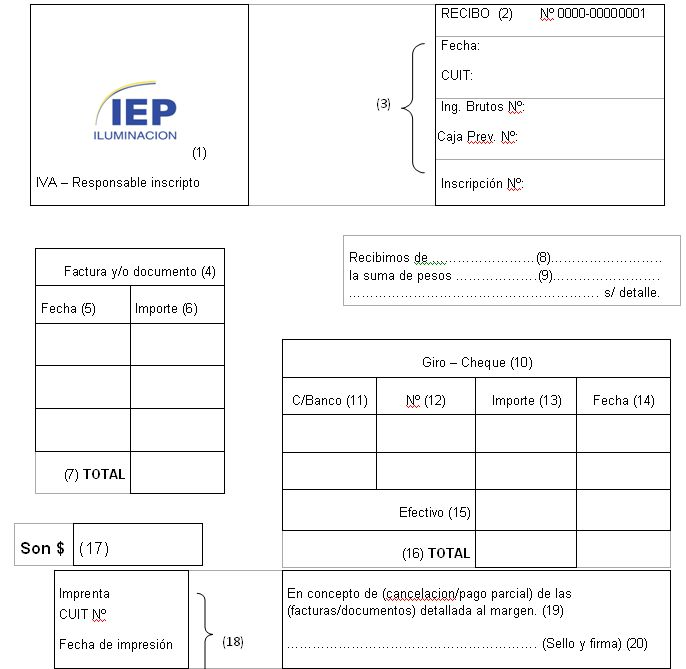
\includegraphics[scale=0.6]{./Images/FormulariosIEP/recibo.jpg}
\end{center}

\begin{itemize}
  \item \textbf{Objetivo:} Servir de comprobante para dejar constancia de la cobranza realizada.
  \item \textbf{Alcance:} Este documento lo confecciona el cobrador al recibir un pago del cliente.
  \item \textbf{Emisor:} Cobrador
  \item \textbf{Cantidad de Copias Emitidas:} 3
  \item \textbf{Sector receptor:} el cliente (original); tesorería el duplicado, cobranzas el triplicado, y el cuadruplicado queda retenido por el cobrador (luego pasa a cobranzas).
 \end{itemize}
 
\subsubsection{Descripci\'on campos Recibo}
\begin{enumerate}
\item Identificación del emisor (datos de la empresa: Razón social, dirección, Tipo responsable IVA inscripto)
\item Nº recibo prenumerados y correlativos.
\item Fecha de emisión, Nº Cuit, Nº ingresos brutos, caja previsional, inscripción.
\item Aplicación de la cobranza (Tipo: Factura y/o documento, nota de crédito, nota de débito).
\item Fecha Vencimiento
\item Importe en pesos
\item Total en pesos
\item Razon social
\item Importe en letras (expresado en pesos)
\item Detalle de la cobranza (Tipo: giro-cheque, efectivo, documento).
\item C/Banco
\item Nº documento
\item Importe en pesos
\item Fecha Vencimiento
\item Efectivo en pesos.
\item Total en pesos.
\item Importe total en pesos.
\item Datos de la  imprenta (Imprenta, apellido y nombre o razón social, Nº Cuit,  fecha de impresión).
\item En concepto de (cancelación / pago  parcial) de las (facturas / documentos) detalladas al margen.
\item Sello y firma del proveedor.
\end{enumerate}


\pagebreak
\section{Normas de Control Interno de Cobranzas}

\begin{large}
\textbf{Normas específicas de Cobranzas:}
\end{large}

\begin{itemize}

\item \textbf{Control de los recibos:}
Los recibos, provisorios o definitivos, deben estar encuadernados en talonarios, prenumerados,
utilizarse en forma correlativa y quedar una copia adherida al talonario. Los recibos también están sujetos a
las disposiciones de la DGI.
También es importante el control de los talonarios recibidos de la imprenta y que se encuentren bajo
custodia de un responsable, que podría ser el Tesorero. Toda entrega de nuevos talonarios a quienes los
utilizan debe hacerse mediante constancia escrita con el objeto de deslindar responsabilidades.

\item \textbf{Rendición diaria de la cobranza:}
Cuando las cobranzas son realizadas mediante una gestión externa, se debe evitar que los valores
recaudados sean utilizados para fines ajenos a los de la empresa y además, permitir la pronta
disponibilidad de los fondos. Los cobradores deben rendir diariamente sus cobranzas o, en su defecto,
depositar directamente en la cuenta bancaria de la empresa el producto de las mismas.

\item \textbf{Apertura de la correspondencia:}
Debe ser abierta por un funcionario responsable o su secretaria. En el caso de que se utilice esta
modalidad de cobranza, quien concentra la responsabilidad de recepción y distribución de la
correspondencia confeccionará una planilla con el detalle de los valores recibidos, y la emisión del recibo
quedará a cargo de Tesorería. Tesorería recibe los valores acompañados de una planilla de cobranza,
como en el caso de la cobranza efectuada por un cobrador.

\item \textbf{Control sobre los valores recibidos:}
Se debe controlar adecuadamente que los valores recibidos cumplan las condiciones establecidas
para ser recibidos, en lo referente a su confección, firmas autorizantes fechas, que sean originales no
falsificados, etc. en todas las condiciones establecidas al respecto.
Para evitar que alguien pueda apoderarse de un cheque, es importante que, al momento de su
recepción, se le coloque al dorso una leyenda que restrinja su utilización, tal como únicamente para
depositar en la cuenta de (nombre de la empresa). ( en caso de que no se descuenten o endosen a
terceros)
Las transferencias de dinero o valores deben respaldarse mediante un comprobante que permita
deslindar responsabilidades con respecto a su custodia y además, debe realizarse entre la menor cantidad
de sectores posibles para facilitar el seguimiento.
Para tener un mejor control de las cobranzas y de los fondos ingresados, resulta imprescindible
depositar diariamente en forma integral los valores recibidos, evitando endosos a terceros.

\item \textbf{Concesión de descuentos por pronto pago:}
Con el objeto de evitar posibles fraudes que pudieran cometerse mediante el ingreso a la empresa
de importes inferiores a los realmente cobrados, justificando la diferencia con un descuento concedido, la
concesión de este tipo de descuento debe estar autorizada por un funcionario que pueda hacer uso de esta
atribución.
En caso de que la cobranza sea realizada fuera de la empresa, se puede autorizar al cobrador a
aplicar y calcular los descuentos correspondientes, siempre que ello este debidamente documentado (podrá
estar estipulado en la factura o bien establecido en una norma de cobranzas) y se controle adecuadamente.
Se deben contratar seguros adecuados para resguardar los bienes, tanto fuera de la empresa como dentro
de la misma.

\end{itemize}

